\documentclass[final,t]{beamer}
\mode<presentation>{ \usetheme{Major} }
  \usepackage{times}
  \usepackage{amsmath,amsthm, amssymb, latexsym}
  \boldmath
  \usepackage[english]{babel}


\usepackage{tikz}
\usetikzlibrary{positioning,shadows,arrows,shapes,calc,backgrounds}

\definecolor{forestgreen}{RGB}{34,139,34}
  
  	\usepackage{relsize}
  	\usepackage{multirow}
	%\usepackage{qtree}
	\usepackage{stmaryrd}
	\usepackage{booktabs}
%  \usepackage[font=small,format=plain,labelfont=bf,up,textfont=it,up]{caption}
  	\usepackage[font=scriptsize,labelfont=scriptsize,bf]{caption}
  	\usepackage[latin1]{inputenc}
  	\usepackage[orientation=landscape,size=a1,scale=1.4,debug]{beamerposter}
  	\usepackage{color,listings}
  	\usepackage{calc,xcolor}
        
\definecolor{lightblue}{rgb}{.85,.85,1} % 217 217 255
\definecolor{lightorange}{rgb}{1,.8,.6} % 255 204 153
\definecolor{lightgreen}{rgb}{.77,.91,.5} % 196 232 128
\definecolor{lightyellow}{rgb}{1,.98,.6} % 255 250 153
  	
\newsavebox\CBox
\newenvironment{ColorBox}[3][black]{%
\par\noindent
\def\borderColor{#1}\def\bgColor{#2}
\begin{lrbox}{\CBox}
\minipage{#3-2\fboxsep-2\fboxrule}%
}{%
\endminipage\end{lrbox}%
\fcolorbox{\borderColor}{\bgColor}{\usebox\CBox}\par}
  	
\lstset{language=java}
\lstset{breaklines=true}
\lstset{showstringspaces=false}
\lstset{tabsize=3}
\lstset{basicstyle=\ttfamily\scriptsize}
\lstset{breakautoindent=true}
\lstset{postbreak=\space}
%\lstset{commentstyle=\color{XcodeComments}}
%\lstset{keywordstyle=\color{XcodeKeywords}}
%\lstset{stringstyle=\color{XcodeStringstyle}}

  %%%%%%%%%%%%%%%%%%%%%%%%%%%%%%%%%%%%%%%%%%%%%%%%%%%%%%%%%%%%%%%%%%%%%%%%%%%%%%%%%5
  \title{A Pointer-Based File Management System to Reduce Redundency and Storage Overhead}
  \author[Licastro]{Braden D. Licastro}
  \institute{Department of Computer Science, Allegheny College}
  \date[CSRS 2013] {First Annual Computer Science 580 Research Symposium}
  \webpage{http://www.fullforceapps.com/}
  \mail{licastb@allegheny.edu}

  %%%%%%%%%%%%%%%%%%%%%%%%%%%%%%%%%%%%%%%%%%%%%%%%%%%%%%%%%%%%%%%%%%%%%%%%%%%%%%%%%5
\begin{document}
  \begin{frame}{}  
  \vspace*{-6mm}
  	\begin{columns}[t]

%%%%%%%%%%%%%%%%%%%%%%%%%%%%%%%%%%%%%%%%%%%%%%%%%%%%%%%%%%%%%%%%%%%%%      
%
% Left column
%
%%%%%%%%%%%%%%%%%%%%%%%%%%%%%%%%%%%%%%%%%%%%%%%%%%%%%%%%%%%%%%%%%%%%%  
      \begin{column}{.325\linewidth}

	%%%%%%%%%%%%%%%%%%%%%%%%%%%%%%%%%%%
	%
	% Important Contributions
	%
	%%%%%%%%%%%%%%%%%%%%%%%%%%%%%%%%%%%
        %% \begin{alertblock}{\textsc{Important Contributions}}
	%%   \begin{itemize}
	%%   \item Enhanced the Java 6 Standard Edition compiler
	    
	%%   \item Provides its own domain specific language (DSL)
	    
	%%   \item Easily applicable in all Java development environments
			
	%%   \item Effectively reduces mutant generation time to a minimum
	%%   \end{itemize}        
        %% \end{alertblock}        

	%%%%%%%%%%%%%%%%%%%%%%%%%%%%%%%%%%%
	%
	% Motivation
	%
	%%%%%%%%%%%%%%%%%%%%%%%%%%%%%%%%%%%
        \begin{block}{\textsc{Motivation}}

      	  \begin{itemize}
          
            \item There was approximately 2.8 billion terabytes of data in the world as of January 2012.

            \item Approximately 5\% of the world's data is redundant.
            
            \item Collectively, businesses spend \$1.8 trillion annually to store data.
            
            \item By removing even 1\% of the redundant data, that is an annual savings of \$18 billion dollars.
          
          \end{itemize}

        \end{block}

	%%%%%%%%%%%%%%%%%%%%%%%%%%%%%%%%%%%
	%
	% Types of file systems
	%
	%%%%%%%%%%%%%%%%%%%%%%%%%%%%%%%%%%%
	\begin{block}{\textsc{What is a file system?}}

          \begin{figure}			
  	    \centering
            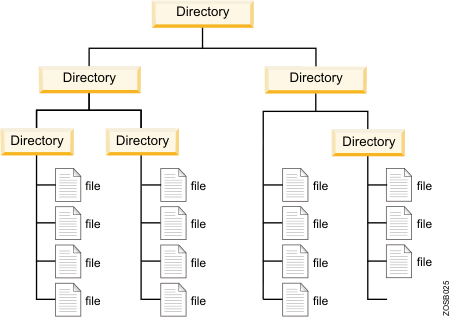
\includegraphics[scale=1.5]{fs.png}
            \vspace*{.05in}
	    \caption{Example file system tree structure.}

	  \end{figure}
          \vspace*{-.2in}
		File systems are a type of data store that can be used to store, retrieve, and update a set of files on a hard disk.
   	\end{block}

	%%%%%%%%%%%%%%%%%%%%%%%%%%%%%%%%%%%
	%
	% Test Suite Reduction's Role
	%
	%%%%%%%%%%%%%%%%%%%%%%%%%%%%%%%%%%%
   	\begin{block}{\textsc{Types of file systems}}

          \begin{itemize}
          
            \item ntfs

            \item exfAT
            
            \item fat
            
            \item fat32
            
            \item ext3
            
          \end{itemize}         
		  
          \begin{itemize}

            \item Why so many? Each file system is designed and tailored for a specific need.
            
            \item All-inclusive file system would not be user friendly and would more than likely become bloated and unreliable.
          
          \end{itemize}         

	\end{block}
      \end{column}   
      
%%%%%%%%%%%%%%%%%%%%%%%%%%%%%%%%%%%%%%%%%%%%%%%%%%%%%%%%%%%%%%%%%%%%%      
%
% Center column
%
%%%%%%%%%%%%%%%%%%%%%%%%%%%%%%%%%%%%%%%%%%%%%%%%%%%%%%%%%%%%%%%%%%%%%
      \begin{column}{.325\linewidth}
   		
	%%%%%%%%%%%%%%%%%%%%%%%%%%%%%%%%%%%
	%
	% Datatabase-Aware Coverage
	%
	%%%%%%%%%%%%%%%%%%%%%%%%%%%%%%%%%%%
	\begin{block}{\textsc{Related Work}}

		\textbf{A Fast Filtering Scheme for large Database Cleansing \cite{a1}}
          \begin{itemize}
          
            \item Database focused algorithms

            \item Data redundency reduction
            
            \item Matches data, not entire files
            
            \item Completely removes duplicates from database
          
          \end{itemize} 
          
          \begin{figure}			
  	    \centering
            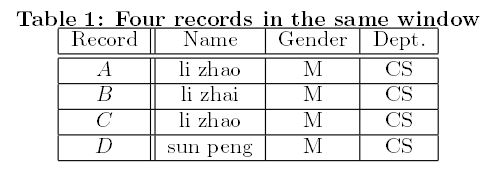
\includegraphics[scale=1.8]{duptable.JPG}
            \vspace*{.05in}
            
	  \end{figure}          

	\end{block}
		
	%%%%%%%%%%%%%%%%%%%%%%%%%%%%%%%%%%%
	%
	% Datatabase-Aware Coverage
	%
	%%%%%%%%%%%%%%%%%%%%%%%%%%%%%%%%%%%
	\begin{block}{\textsc{Related Work}}

		\textbf{A Data De-duplication Access Framework for Solid State Drives \cite{a2}}
          \begin{itemize}
          
            \item Algorithms tuned for solid state drives running on computing cluster

            \item Finds candidate duplciates from calculated scores
            
            \item Minimal read and write calls needed to operate
                
          \end{itemize} 
          
          \begin{figure}			
  	    \centering
            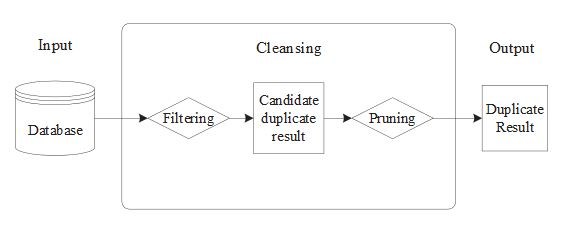
\includegraphics[scale=1.4]{duplicate.JPG}
            \vspace*{.05in}
	    \caption{Authors process for finding and processing duplicates.}
            
	  \end{figure}          

	\end{block}
	
	%%%%%%%%%%%%%%%%%%%%%%%%%%%%%%%%%%%
	%
	% The Empirical Results
	%
	%%%%%%%%%%%%%%%%%%%%%%%%%%%%%%%%%%%
        \begin{block}{\textsc{Challenges}}
          \begin{itemize}

            \item Initial setup time costs when hashing user files.

            \item Keep performance costs to a minimum when interacting with system.

            \item Implementing a web based environment for file system interaction.
            
            \item Verify that pointers all function as intended and file modifications drop pointer accordingly.

          \end{itemize}

          \vspace*{.2in}    
          
	\end{block}

	\end{column}

%%%%%%%%%%%%%%%%%%%%%%%%%%%%%%%%%%%%%%%%%%%%%%%%%%%%%%%%%%%%%%%%%%%%%      
%
% Right column
%
%%%%%%%%%%%%%%%%%%%%%%%%%%%%%%%%%%%%%%%%%%%%%%%%%%%%%%%%%%%%%%%%%%%%%      		
      \begin{column}{.325\linewidth}	
		
	%%%%%%%%%%%%%%%%%%%%%%%%%%%%%%%%%%%
	%
	% The Empirical Results
	%
	%%%%%%%%%%%%%%%%%%%%%%%%%%%%%%%%%%%
        \begin{block}{\textsc{Implementation}}
          \begin{itemize}

            \item Create or modify existing file system

            \item Hash files usign MD5 hashing algorithm to allow checking for matches.

            \item Remove duplicate files and replace duplicate with pointer referring to the parent copy

            \item Overwrite opened pointer with modified file to prevent overwriting a needed original.

            \item Restrict file database to non-system files.

          \end{itemize}

          \vspace*{.2in}    
              
          \begin{figure}			
  	    \centering
            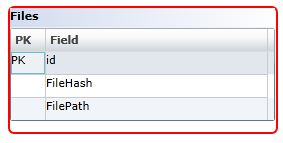
\includegraphics[scale=2.2]{schema.JPG}
            \vspace*{.05in}
            
	  \end{figure}
	\end{block}
	
		%%%%%%%%%%%%%%%%%%%%%%%%%%%%%%%%%%%
	%
	% The Empirical Results
	%
	%%%%%%%%%%%%%%%%%%%%%%%%%%%%%%%%%%%
        \begin{block}{\textsc{Method of Evaluation}}
          \begin{itemize}

            \item Measure space saved by removing duplicates including size of the database in calculations.

            \item Monitor performance impact of running implemented project vs OOB file system

            \item View file tree structure, starting with a set structure and compare to tree after removing duplicates.
            
            \item Verify that pointers all function as intended and file modifications drop pointer accordingly.

          \end{itemize}

          \vspace*{.2in}    
          
	\end{block}
	
	%%%%%%%%%%%%%%%%%%%%%%%%%%%%%%%%%%%
	%
	% Future Work
	%
	%%%%%%%%%%%%%%%%%%%%%%%%%%%%%%%%%%%				
	\begin{alertblock}{\textsc{Future Work}}
		\bibliographystyle{plain}
		\bibliography{finalbib}
	\end{alertblock}
      \end{column}
      
	\end{columns}
  \end{frame}
\end{document}
